% =====================================================================
% SECTION: Droop Control Design and Gain Selection
% Sources of truth:
%   controller_design/system_model.md  (§2, §3, §4, §8)
%   teensy_controller/teensy_controller.ino  (lines 451-468, 2180-2190, 2760-2840)
%   CLAUDE.md §5, §7, addendum 2026-07-10 and 2026-07-11
% =====================================================================
\section{Droop Control Design and Gain Selection}
\label{sec:droop}

\subsection{Design Ethos: Power Sharing Without a Custom Power Stage}
\label{sec:droop:ethos}

% NOTE(author): rewrite this paragraph in the paper's voice; the argument is right
% but the prose is engineer-terse. Emphasise the "commodity silicon + analog
% perturbation" framing, which is the paper's actual contribution claim.
The power-sharing objective for a hybrid fuel-cell/battery vehicle is to place a commanded
fraction $\alpha_{req}$ of the bus current on the fuel cell and the remainder on the
battery, continuously and under load transients. The conventional route is a
purpose-designed dual-input converter with a shared, digitally arbitrated current loop.
This work deliberately takes the opposite route: both sources are boosted by
\emph{unmodified, off-the-shelf} converters (Texas Instruments TPS61288, constant-off-time
peak-current-mode boost), and sharing is imposed by \emph{perturbing each regulator's
feedback node} with a signal proportional to that regulator's own output current. Each
converter therefore behaves as a Th\'evenin source with an electronically programmable
output resistance, and the two sources share current by classical droop --- but with a
droop coefficient the microcontroller can rewrite at any instant.

The advantages that motivate this choice are practical rather than theoretical:

\begin{enumerate}
  \item \textbf{No custom power stage.} The converters keep their datasheet compensation,
        protection, soft-start, and thermal behaviour. Nothing in the high-current path is
        bespoke, so the failure modes are the vendor's characterised ones.
  \item \textbf{The fast loop stays analog.} Current sensing, scaling, and injection are
        continuous-time hardware; the digital controller only \emph{trims a coefficient}.
        Sharing does not collapse if the MCU is late, and the loop is not sampled at the
        converter's switching time scale.
  \item \textbf{Graceful degradation.} With the digital-to-analog converters parked at a
        fixed code the board is still a working, statically drooped parallel supply. The
        control law is an enhancement, not a prerequisite for operation.
\end{enumerate}

The per-channel signal chain that realises this is fixed by the board and is shown in
Figure~\ref{fig:droop-chain}: the channel's output current is measured by an INA253A1
integrated shunt amplifier, scaled by a 12-bit AD5443 multiplying DAC (MDAC) operating in
voltage-switching mode, buffered and amplified by an OPA197, and injected through a
resistor into the boost converter's feedback divider node.

\begin{figure}[H]
  \centering
  % FIGURE FILE: controller_design/figures/droop_signal_chain.svg
  % (convert to PDF for LaTeX: inkscape --export-type=pdf droop_signal_chain.svg)
  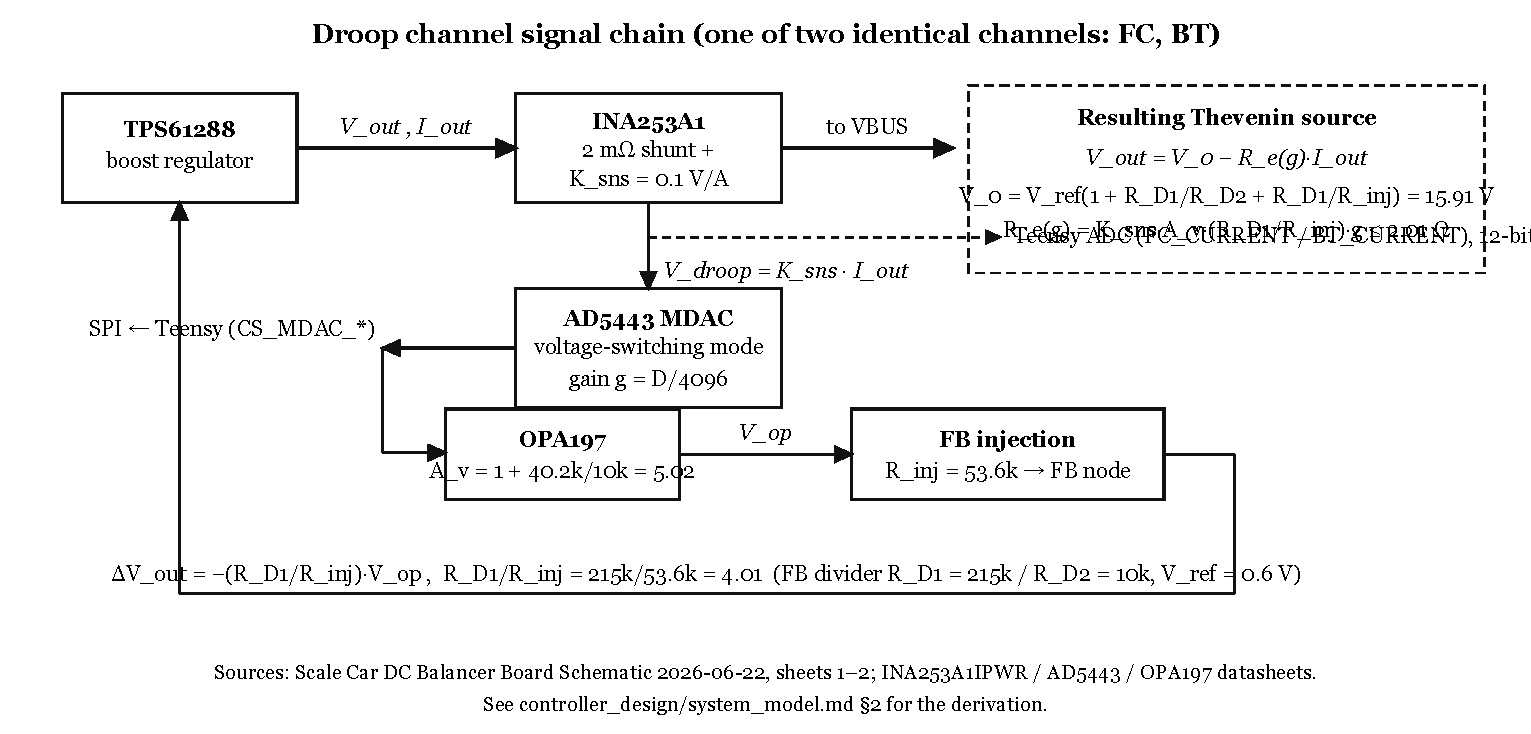
\includegraphics[width=\linewidth]{Figures/droop_signal_chain.pdf}
  \caption{Per-channel droop signal chain. The channel output current is sensed by the
  INA253A1 ($K_{sns}=0.1$\,V/A), scaled by the AD5443 MDAC (gain $g \in [0,4095/4096]$,
  written over SPI), amplified by the OPA197 ($A_v = 5.02$), and injected through
  $R_{inj}=53.6$\,k$\Omega$ into the TPS61288 feedback node
  ($R_{D1}=215$\,k$\Omega$, $R_{D2}=10$\,k$\Omega$). The converter is unmodified; the
  entire droop mechanism is an additive perturbation of its feedback divider.}
  \label{fig:droop-chain}
\end{figure}

\subsection{Droop Equations and the Actuator Mapping}
\label{sec:droop:equations}

\subsubsection{Effective output resistance}

The converter servos its feedback node to $V_{ref}$. Writing KCL at that node (feedback
pin current negligible) with the injected voltage $V_{op}$ gives

\begin{equation}
  \frac{V_{out}-V_{ref}}{R_{D1}} + \frac{V_{op}-V_{ref}}{R_{inj}} = \frac{V_{ref}}{R_{D2}},
  \label{eq:fb-kcl}
\end{equation}

which rearranges into an explicit Th\'evenin form,

\begin{equation}
  V_{out} = \underbrace{V_{ref}\!\left(1 + \frac{R_{D1}}{R_{D2}} + \frac{R_{D1}}{R_{inj}}\right)}_{V_0\ \text{(no-load setpoint)}}
            \;-\; \frac{R_{D1}}{R_{inj}}\,V_{op}.
  \label{eq:thevenin}
\end{equation}

Substituting the measured-current path $V_{op} = A_v\,g\,K_{sns}\,I_{out}$ yields the
programmable output resistance that is the heart of the scheme:

\begin{equation}
  V_{out} = V_0 - R_e(g)\,I_{out},
  \qquad
  \boxed{\;R_e(g) = K_{sns}\,A_v\,\frac{R_{D1}}{R_{inj}}\,g \;=\; R_{e,max}\,g\;}
  \label{eq:re}
\end{equation}

with the numerical values of the as-built board:

\begin{align}
  K_{sns} &= 0.1\ \mathrm{V/A}  && \text{INA253A1 fitted (A3 would be 0.4)}\\ % INA253A1IPWR.pdf; system_model.md §8
  A_v     &= 1 + \tfrac{40.2\,\mathrm{k}}{10\,\mathrm{k}} = 5.02 && \text{op-amp gain}\\ % schematic ROP1/ROP2; system_model.md §8; .ino const float A_v
  R_{D1}/R_{inj} &= \tfrac{215\,\mathrm{k}}{53.6\,\mathrm{k}} = 4.011 && \text{injection attenuation}\\ % system_model.md §2/§8; .ino RD1_OVER_RINJ
  R_{e,max} &= 0.1 \times 5.02 \times 4.011 = \mathbf{2.014\ \Omega} && \\ % system_model.md §8; .ino RE_MAX
  V_0 &= 0.6 \times 26.51 = 15.91\ \mathrm{V} && \text{no-load setpoint} % V_ref=0.6V, TPS61288LRQQR.pdf §7.5; system_model.md §2
\end{align}

% NOTE(author): the RD1 value is a post-manufacturing bodge (237k -> 215k, both channels,
% 2026-07-11, part of the 16 V bus retune). The released schematic still prints 237k.
% Decide whether the paper documents the bodge explicitly or simply reports as-built
% values; recommend a single footnote rather than a digression.
The 12-bit MDAC resolves this into $\Delta R_e = R_{e,max}/4096 = 0.49$\,m$\Omega$ per LSB,
which is far below any effect the current sensing can resolve; MDAC quantisation is
therefore omitted from the linear model.

\subsubsection{Two sources in parallel}

With both channels conducting onto the bus through their ideal-diode switches, and total
load current $I_{tot}$,

\begin{equation}
  V_{bus} = V_{0F} - R_F I_F = V_{0B} - R_B I_B, \qquad I_F + I_B = I_{tot}.
\end{equation}

The design choice that makes this a well-conditioned control problem is to command the two
droop resistances \emph{reciprocally} from a single scalar ratio $r$, using a fixed design
droop scale $k_d$ (denoted \texttt{K\_DROOP} in firmware):

\begin{equation}
  R_F = \frac{k_d}{r}, \qquad R_B = \frac{k_d}{1-r}.
  \label{eq:ratio-map}
\end{equation}

This has the property $R_F \parallel R_B = k_d$ \emph{independently of} $r$: the bus's
aggregate droop stiffness is constant while the split is swept. The resulting share is

\begin{equation}
  \boxed{\;\alpha \;=\; \frac{I_F}{I_{tot}} \;=\; r \;+\; \underbrace{\frac{\Delta V_0\, r(1-r)}{k_d\, I_{tot}}}_{d\ \text{(output disturbance)}}\;}
  \label{eq:share}
\end{equation}

where $\Delta V_0 \equiv V_{0F}-V_{0B}$ is the channel-to-channel no-load setpoint
mismatch. Three consequences drive the controller design: the nominal static gain is
exactly unity ($\alpha = r$); setpoint mismatch enters as an additive output disturbance
that is worst at $r=0.5$ and at light load and scales as $1/k_d$; and the same mismatch
perturbs the plant gain,
$\partial\alpha/\partial r = 1 + \Delta V_0(1-2r)/(k_d I_{tot})$, which is carried into
synthesis as parametric gain uncertainty.

\subsubsection{The actuator mapping --- and a design lesson}
\label{sec:droop:bug}

Combining \eqref{eq:re} and \eqref{eq:ratio-map} gives the mapping the firmware must
implement:

\begin{equation}
  \boxed{\;g_F = \frac{k_d}{R_{e,max}\,r}, \qquad g_B = \frac{k_d}{R_{e,max}\,(1-r)}\;}
  \label{eq:g-map}
\end{equation}

% NOTE(author): this subsection is deliberately a confession. Reviewers of control papers
% reward honestly reported model-vs-hardware defects far more than a clean narrative, and
% it directly motivates why the plant was re-derived from the schematic rather than from
% the existing code. Keep it, but tighten the tone -- it currently reads as a lab notebook.
It is worth reporting that the original firmware did \emph{not} implement
\eqref{eq:g-map}. It used an equivalent-resistance constant $k_{eq}=0.45$\,$\Omega$ and
computed $g = k_{eq}/(r\,K_{sns}A_v)$ --- an expression that models the sense-and-amplify
path but silently \emph{omits the feedback-injection attenuation} $R_{D1}/R_{inj}$, at that
time $237\,\mathrm{k}/53.6\,\mathrm{k}=4.42$. The consequence is not a mild gain error. The
commanded gain becomes $g_F = 0.45/(0.502\,r) = 0.896/r$, which exceeds unity for every
$r < 0.896$; the SPI write routine clamps to full scale; and therefore across essentially
the whole commanded range \emph{both} MDACs sat pinned at $g=1$, giving
$R_F = R_B = R_{e,max}$ and a fixed $50/50$ share.

The control-theoretic reading is the important one: the loop was not badly tuned, it was
operating on a \textbf{zero-gain plant}. Any $\partial\alpha/\partial r$ was identically
zero over the operating range, so no choice of controller gains --- and the legacy design
used $K_p = K_i = 1$, which \eqref{eq:share} makes superficially plausible since the
nominal plant gain is unity --- could have produced closed-loop share authority. The defect
is invisible to a firmware unit test (the code computes what it says it computes), invisible
to a step response at fixed load (the share is stable, merely uncontrolled), and only
becomes obvious when the actuator mapping is re-derived from the schematic and the
saturation limit $g \le 1$ is checked explicitly. The lesson we draw, and recommend, is
that \emph{an actuator-range audit against the physical hardware constants should be a
mandatory step before any plant identification}: a saturated actuator and a well-behaved
plant are indistinguishable in closed-loop data.

\subsection{Gain Selection and the PCB Constraints It Imposed}
\label{sec:droop:gains}

% NOTE(author): this is the section that answers the "co-design" claim in the abstract.
% Make explicit that the resistor values were chosen *because* of the droop gain decision,
% not the other way round.
The droop gain choice is not a purely digital decision. Because $R_e$ is realised in
analog hardware, selecting $k_d$ simultaneously fixes MDAC range utilisation, op-amp
headroom, and the achievable share authority --- and those in turn dictated component
values on the PCB. The binding constraints are the following.

\paragraph{Constraint 1: MDAC saturation sets the ratio span.}
Since $g \le 1$, \eqref{eq:g-map} bounds the usable ratio range by
$k_d \le R_{e,max}\cdot\min(r_{min},\,1-r_{max})$. This is a direct trade of \emph{droop
stiffness against control authority}:

\begin{table}[H]
  \centering
  \caption{Droop-scale bound versus commanded ratio span, at $R_{e,max}=2.014\ \Omega$.
           The middle row is the shipped design point.}
           % Source: system_model.md §4 trade table (values rescaled to the 215k RD1 bodge)
  \label{tab:kd-tradeoff}
  \begin{tabular}{lcl}
    \toprule
    Ratio span $[r_{min},r_{max}]$ & max $k_d$ ($\Omega$) & Character \\
    \midrule
    $[0.10,\,0.90]$ & 0.201 & Wide authority, weak droop \\
    $\mathbf{[0.15,\,0.85]}$ & \textbf{0.302} & \textbf{Shipped: $k_d=0.30\ \Omega$, max $g=0.993$} \\
    $[0.20,\,0.80]$ & 0.403 & Strong droop, narrow authority \\
    \bottomrule
  \end{tabular}
\end{table}

% NOTE(author): 0.30 is still TODO(calibrate) in firmware pending the CAL-1/CAL-3 bench runs.
% Either report it as provisional or hold the paper's number until bench data lands.
The selected point is $k_d = 0.30\ \Omega$ with clamps
$[\texttt{DROOP\_R\_MIN},\texttt{DROOP\_R\_MAX}] = [0.15,\,0.85]$, leaving $0.7\%$ of MDAC
range as margin against component tolerance. Larger $k_d$ suppresses the mismatch
disturbance $d \propto 1/k_d$ but costs bus regulation --- the droop sag at $r=0.5$ is
$k_d I_{tot}$, i.e.\ $1.8$\,V at $6$\,A --- and narrows the reachable share range. Smaller
$k_d$ widens authority but lets the $\Delta V_0$ mismatch dominate the share error.

\paragraph{Constraint 2: the injection resistor sets $R_{e,max}$ \emph{and} the bus setpoint
simultaneously.}
$R_{inj}$ appears in both \eqref{eq:thevenin} and \eqref{eq:re}: it attenuates the
injected droop signal (setting the ceiling $R_{e,max}$) and it also loads the feedback
divider (shifting the no-load setpoint $V_0$). It cannot be chosen for droop range alone.
The board's $R_{inj} = 53.6$\,k$\Omega$ against $R_{D1} = 215$\,k$\Omega$ yields
$R_{e,max}=2.014\ \Omega$ --- comfortably above the $0.302\ \Omega$ requirement, i.e.\ the
design deliberately uses only $\approx 15\%$ of the available droop authority at the range
centre so that the whole span stays clear of MDAC saturation. This coupling was also the
mechanism by which a later system-level decision propagated back into the droop design: the
$16$\,V bus retune (undertaken for converter overshoot headroom, unrelated to sharing)
changed $R_{D1}$ from $237$\,k to $215$\,k$\Omega$, which moved $R_{e,max}$ from
$2.220\ \Omega$ to $2.014\ \Omega$ and required $k_d$ to be reduced from $0.33$ to
$0.30\ \Omega$ to preserve the $g\le1$ bound.
% Source: .ino changelog lines 75-82; system_model.md §2 and §8.

\paragraph{Constraint 3: sense gain versus op-amp headroom.}
The OPA197 is supplied from the board's $5$\,V rail (a post-manufacturing change from
$3.3$\,V), so its output ceiling is $\approx 4.9$\,V. The injected signal is
$V_{op} = A_v g K_{sns} I_{out}$, so the headroom limit is
$g\,I_{out} \le 4.9/(5.02\times0.1) = 9.8$\,A --- non-binding for this vehicle, whose
per-channel current stays below roughly $3$\,A. Note, however, that this margin is a
\emph{consequence of a component substitution error}: the design intended the INA253A3
($K_{sns} = 0.4$\,V/A) and the INA253A1 ($0.1$\,V/A) was fitted. The A3 part would have
raised $R_{e,max}$ fourfold (making the MDAC range constraint far looser) but would equally
have reduced the headroom ceiling to $2.4$\,A$\cdot$g, which \emph{would} have been binding
at peak current. The firmware carries $K_{sns}$ as an explicit named constant precisely so
this variant choice remains a single-line change if the board is respun.
% Source: CLAUDE.md §5 and §7; system_model.md §8; .ino const float K_sns

\paragraph{Constraint 4: the clamps are the anti-windup boundary.}
Because the ratio clamps $[0.15,0.85]$ are the true actuator saturation, they --- not an
arbitrary controller output limit --- define the anti-windup boundary for the outer
share controller. The clamp is applied in the firmware before the mapping
\eqref{eq:g-map} is evaluated, so the commanded MDAC gain is guaranteed to satisfy
$g \le 1$ by construction and the digital controller never operates against a hidden
hardware limit. The legacy $[0.01,\,0.99]$ clamps, which permitted the saturated regime of
Section~\ref{sec:droop:bug}, were removed from the droop path.

Figure~\ref{fig:control-loop} places these elements in the linearised design loop used for
synthesis, showing where the mismatch disturbance $d$ and the current-sense noise $n$ enter.

\begin{figure}[H]
  \centering
  % FIGURE FILE: controller_design/figures/control_loop_model.svg
  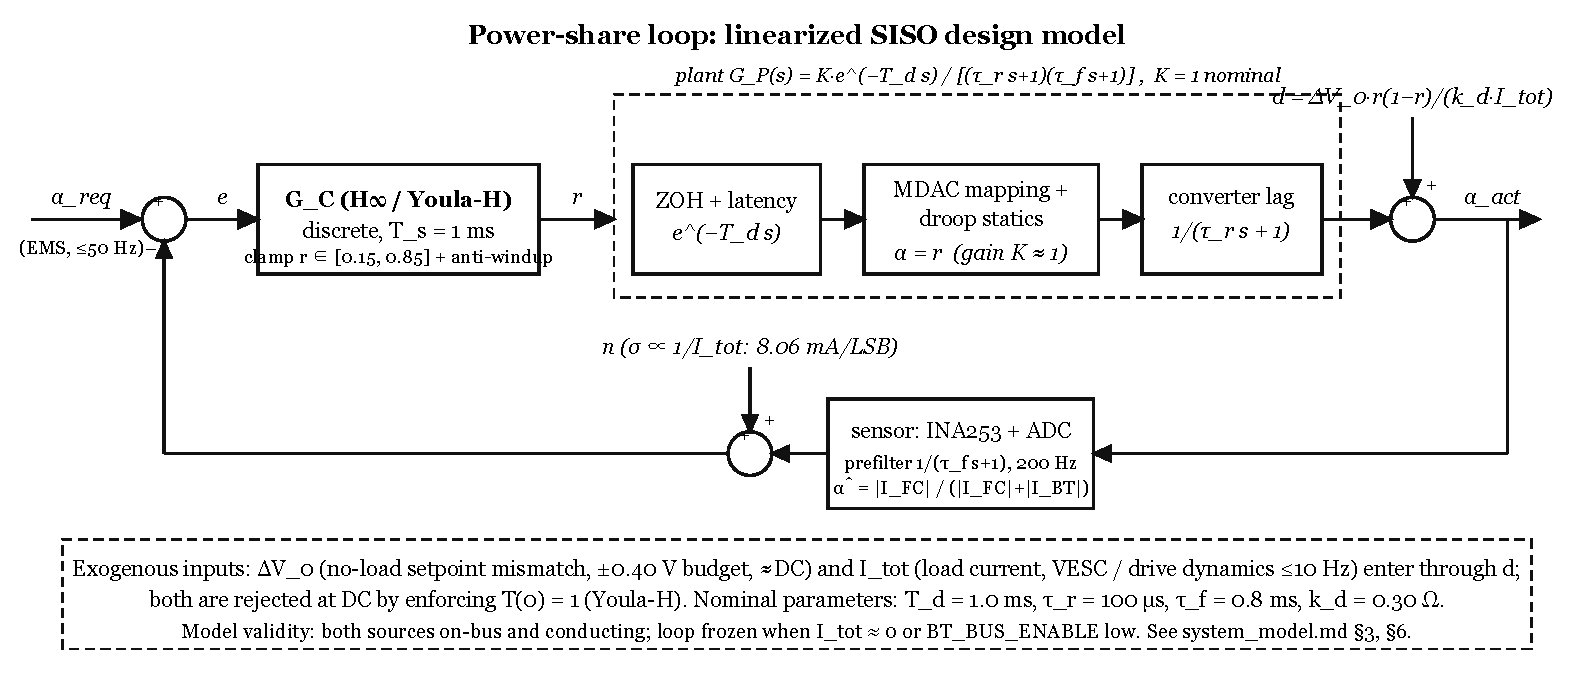
\includegraphics[width=\linewidth]{Figures/control_loop_model.pdf}
  \caption{Linearised SISO share-control loop. The controller commands the droop ratio $r$;
  the actuator mapping $g=k_d/(R_{e,max}r)$ and its clamp to $[0.15,0.85]$ form the
  saturation element. The plant reduces to a near-unity static gain in series with the
  converter lag $\tau_r$, the measurement prefilter $\tau_f$, and the dominant loop delay
  $T_d$. Setpoint mismatch $\Delta V_0$ enters as the additive output disturbance
  $d = \Delta V_0 r(1-r)/(k_d I_{tot})$; current-sense quantisation enters as output noise
  $n$ with variance scaling as $1/I_{tot}$.}
  \label{fig:control-loop}
\end{figure}

% =====================================================================
% PLANNING NOTES  (delete before submission)
% =====================================================================
% SCOPE / STATUS
% - This is a planning draft. Every number is traceable to
%   controller_design/system_model.md §2/§4/§8 or to the constants block in
%   teensy_controller/teensy_controller.ino (~lines 451-468). Do not edit numbers here
%   without editing system_model.md; that file is the declared source of truth.
%
% NUMBERS THAT ARE STILL PROVISIONAL (marked TODO(calibrate) in the repo)
% - k_d = 0.30 ohm  ..... bench decision pending (CAL-1 / CAL-3 in system_model.md §9).
%                         If it moves, Table \ref{tab:kd-tradeoff}, the 1.8 V sag figure,
%                         and the "0.7% MDAC margin" claim all change, AND the Youla-H
%                         controller coefficients must be regenerated (never hand-edited).
% - Delta V0 = +/-0.40 V  budgeted by tolerance RSS, not yet measured per board. The
%                         disturbance magnitudes quoted downstream depend on it.
% - tau_r = 100 us ...... lumped estimate; step test pending.
% - V_ref = 0.6 V ....... datasheet-verified (TPS61288 DS §7.5) but per-board value
%                         still to be measured in CAL-1.
%
% VERSION HAZARD -- READ BEFORE REUSING TEXT
% - Two sets of droop constants exist in the project history:
%     pre-retune  (RD1 = 237k): RE_MAX = 2.220 ohm, K_DROOP = 0.33, bound 0.3329
%     as-built    (RD1 = 215k): RE_MAX = 2.014 ohm, K_DROOP = 0.30, bound 0.3020
%   This section uses the AS-BUILT set throughout and mentions 2.220/0.33 only in
%   Constraint 2 as the superseded value. Earlier drafts and slide decks may quote the
%   pre-retune numbers. Cross-check any imported figure.
% - The released schematic (2026-06-22) still prints RD1 = 237k and RC-BT = 27.4k. Both
%   were bodged post-manufacturing. If a schematic excerpt is reproduced as a figure it
%   must carry a correction note or the numbers will contradict this section.
%
% FIGURES
% - Both figures exist as SVG in controller_design/figures/. LaTeX needs PDF:
%     inkscape --export-type=pdf droop_signal_chain.svg control_loop_model.svg
%   then copy into Figures/. Confirm the SVGs were regenerated after the 215k bodge --
%   if they annotate 237k they are stale.
% - Consider a third figure: measured alpha vs commanded r, overlaying the saturated
%   legacy mapping (flat at ~0.5) against the corrected mapping (slope ~1). That single
%   plot carries the Section \ref{sec:droop:bug} argument better than the prose does. Data
%   comes from the CAL-1 open-loop sweep (State 98 'O' command) -- NOT YET COLLECTED.
%
% PROSE TO REWRITE (see inline % NOTE markers)
% - Opening of \ref{sec:droop:ethos}: too terse, needs the paper's framing of the contribution.
% - \ref{sec:droop:bug}: currently reads as a lab notebook. Keep the honesty, raise the register.
% - \ref{sec:droop:gains} preamble: must land the hardware/control co-design claim explicitly.
%
% CROSS-REFERENCES TO WIRE UP
% - Constraint 4 -> the anti-windup discussion in the controller synthesis section.
% - Eq \eqref{eq:share} gain-uncertainty term -> the plant uncertainty set K in [0.75,1.25]
%   (widening to [0.55,1.45] at the ratio-span edges) used for synthesis.
% - The MDAC quantisation dismissal -> the noise budget section (system_model.md §5b).
%
% DELIBERATELY OUT OF SCOPE HERE
% - Converter-loop dynamics / tau_r justification (system_model.md §6e) and the
%   full-order validation (full_order_validation.md) belong in the plant-model section.
% - The RC-BT 27.4k -> 61.2k compensator bodge is a converter-symmetry issue, not a droop
%   gain issue; mention it only where the shared tau_r assumption is defended.
% =====================================================================
